%%%%%%%%%%%%%%%%%%%%%%%%%%%%%%%%%%%%%%%%
% basic elements

\documentclass[12pt]{article}
\usepackage[english]{babel}
\usepackage{amsmath,amsthm}
\usepackage{amsfonts}
\usepackage{makecell}
\usepackage{graphics}
\usepackage{graphicx}
\usepackage{fancyhdr}
\usepackage{ifthen}
\usepackage{wrapfig}
\usepackage{array}
\usepackage{colortbl}
\usepackage{fullpage}
\usepackage[table]{xcolor}
\usepackage{subfigure}
\usepackage{caption}
\usepackage{float}
\usepackage{ctex}
\usepackage{appendix}
\usepackage{shorttoc}
\usepackage{pagenote}
\usepackage{setspace}
\usepackage{geometry}
\usepackage{indentfirst}
\usepackage{fullpage}
\usepackage{booktabs}
\usepackage{multirow}
\usepackage{longtable}
\usepackage{minipage-marginpar}
\usepackage{hyperref}
\usepackage{palatino}
\usepackage{setspace}
\usepackage{subfigure}
\usepackage{picinpar}
\usepackage{newtxtext}
\usepackage{amsmath,amssymb,amsthm}
\usepackage{extarrows}
\usepackage{algorithm}
\usepackage{algorithmic}
\usepackage{paralist}
\usepackage{newtxmath} % must come after amsXXX

% Replace ABCDEF in the next line with your chosen problem
% and replace 111111 with your Team Control Number
% and replace abcdef with your Title
% and replace 123456 with the number of pages of your essay
\newcommand{\Problem}{A}
\newcommand{\Team}{{22091106}}
\newcommand{\Title}{{Smart Lamppost Deployment}}
\newcommand{\wholepages}{18}
\title{\Huge\textbf{\Title}}
\author{Team\#\Team}
\date{\today}

%%%%%%%%%%%%%%%%%%%%%%%%%%%%%%%%%%%%%%%%
% set up of theorems

\newtheorem{thm}{Theorem}[section]
\newtheorem{cor}[thm]{Corollary}
\newtheorem{lem}[thm]{Lemma}
\newtheorem{prop}[thm]{Proposition}
\theoremstyle{definition}
\newtheorem{defn}[thm]{Definition}
\theoremstyle{remark}
\newtheorem{rem}[thm]{Remark}
\numberwithin{equation}{section}
\newtheorem{theorem}{Theorem}
\newtheorem{corollary}[theorem]{Corollary}
\newtheorem{lemma}[theorem]{Lemma}
\newtheorem{definition}{Definition}

%%%%%%%%%%%%%%%%%%%%%%%%%%%%%%%%%%%%%%%%
% setup of page length and script size

\setlength{\belowcaptionskip}{9pt}
\setlength{\abovecaptionskip}{9pt}
\setlength{\headsep}{0.4in}
\setlength{\headheight}{14.5pt}
\captionsetup{font={footnotesize}}
\renewcommand{\baselinestretch}{1.02}
\setlength{\parskip}{0.28em}
\geometry{bottom=1in}

%%%%%%%%%%%%%%%%%%%%%%%%%%%%%%%%%%%%%%%%
% set up of page style

\pagestyle{fancy}
\fancyhead[L]{Team\ \#\Team}
\fancyhead[C]{\Title}
\fancyhead[R]{Page \thepage \ of \wholepages}
\fancyfoot{}

%%%%%%%%%%%%%%%%%%%%%%%%%%%%%%%%%%%%%%%%
% hyphenation

\tolerance=1
\emergencystretch=\maxdimen
\hyphenpenalty=10000
\hbadness=10000

\hypersetup{hidelinks} 
\hypersetup{
	colorlinks=false,
	linkcolor=black,
	citecolor=black,
	anchorcolor=black
}
%%%%%%%%%%%%%%%%%%%%%%%%%%%%%%%%%%%%%%%%
% biblography
\bibliographystyle{plain}
% \usepackage{url}
% \def\UrlBreaks{[\do\A\do\B\do\C\do\D\do\E\do\F\do\G\do\H\do\I\do\J\do\K\do\L\do\M\do\N\do\O\do\P\do\Q\do\R\do\S\do\T\do\U\do\V\do\W\do\X\do\Y\do\Z\do\[\do\\\do\]\do\^\do\_\do\`\do\a\do\b\do\c\do\d\do\e\do\f\do\g\do\h\do\i\do\j\do\k\do\l\do\m\do\n\do\o\do\p\do\q\do\r\do\s\do\t\do\u\do\v\do\w\do\x\do\y\do\z\do\.\do\@\do\\\do\/\do\!\do\_\do\|\do\;\do\>\do\]\do\)\do\,\do\?\do\'\do+\do\=\do\#}
%%%%%%%%%%%%%%%%%%%%%%%%%%%%%%%%%%%%%%%%
% end of the beginning part
\begin{document}
	\DeclareGraphicsExtensions{.pdf, .jpg, .tif, .png}
	\thispagestyle{empty}
	\vspace*{-16ex}
	% MCM/ICM Template
	% \centerline{\begin{tabular}{*3{c}}
			%	\parbox[t]{0.3\linewidth}{\begin{center}\textbf{Problem Chosen}\\ \Large \Problem\end{center}}
			%	& \parbox[t]{0.3\linewidth}{\begin{center}\textbf{2020\\ MCM \\ Summary Sheet}\end{center}}
			%	& \parbox[t]{0.3\linewidth}{\begin{center}\textbf{Team Control Number}\\ \Large Team \# \Team\end{center}}	\\
			%	\hline
			%\end{tabular}}
	
	% HiMCM/IMMC Template
	\begin{center}
		\centerline{\begin{tabular}{p{\linewidth}<{\centering}}
				\small Team Control Number \\
				\huge \textbf{\Team} \\
				\small Problem Chosen \\
				\huge \textbf{\Problem} \\
				\textbf{2022} \\
				\small \textbf{IMMC} \\
				\small \textbf{Summary Sheet} \\
				\hline
		\end{tabular}}
	\end{center}
	%%%%%%%%%%% Begin Summary %%%%%%%%%%%%%%%%%%
	% Enter your summary here replacing the (red) text
	% Replace the text from here ...
	\qquad
	\par
	Nowadays, with the rapid development of autonomous driving technology, the establishment of an autonomous driving system will no longer be an absurd idea. In this system, connections can be built between the autonomous driving cars, the smart lampposts installed with sensors and communication units and the cloud server. Therefore we need to carry out a plan which will make the transportation system easier and create an indicator system to evaluate the smart lamppost modification plans.
	
	In the first model, we find out the factors that are related to evaluating a lamppost modification plan. We mainly discuss how to calculate the index which is affected by cost, coverage rate of LiDAR and the importance of each road. Afterwards, we make some plans about the measure of coverage rate in different situations.
	
	In the second model, our goal is to establish an overall optimal configuration of all lampposts within a certain area. Instead of simply simulating all measures, we took a more natural Q-learning approach under the thought of greedy algorithms. The machine-learning process, which relied merely on the mathematical index of a given distribution as shown in the first model, gradually narrowed the result till a fixed distribution. In order to confirm the accuracy of the algorithm, we randomly altered certain sets of lampposts and withdrew the consequent changes in variables. After that, we chose the uniformity of lamppost points as the independent variable and conducted a sensitivity analysis, which, after eliminating certain anomalous data, proved that the results were accurate enough. Out of considerations of dual confirmation, we also checked that the results turned out to be optimal.We did a sensitivity analysis on the model, and found some issues where it cannot evaluate correctly.
	
	Last, we evaluated the plan using the model built in the first part. With the help of Python packages \textit{Shapely} and \textit{Matplotlib}, we managed to calculate the coverage area and coverage rate of our plan in the second part. Probable explanations are raised, and we developed a dynamic model to solve the problem. We also made a dynamic model to simulate the process of WiFi connection using the Hungarian Algorithm.

	% to here
	%%%%%%%%%%% End Summary %%%%%%%%%%%%%%%%%%%
	\thispagestyle{empty}
	\maketitle
	\thispagestyle{empty}
	\newpage
	%%%%%%%%%%%%%%%%%%%%%%%%%%%%%%%%%%%%%%%%
	\clearpage
	\thispagestyle{empty}
	% Uncomment the next line to generate a Table of Contentsr%r%\shortableofcontents{Contents}{2}
	\tableofcontents % Uncomment this line to update the Contents
	\newpage
	\pagestyle{fancy}
	\setcounter{page}{1}
	% Begin your paper here
	%%%%%%%%%%%%%%%%%%%%%%%%%%%%%%%%%%%%%%%%
	
	\newpage
	\section{Introduction}
		\subsection{Background}
		Nowadays, with the rapid development of autonomous driving technology, building an automatic driving system will no longer be a ridiculous thought. Based on recent technology, autonomous driving technology has begun to move from partial driving at the L2 level to conditional driving automation at the L3 level.
		
		According to the degree of automation of the vehicle\cite{Autonomous Driving Levels}, when the system cannot withstand the working conditions, the driver needs to take over the malfunctioning vehicle. After activating the automatic driving system, the vehicle itself can complete tasks such as steering, acceleration, deceleration, and reaction. The status detection and reaction are carried out under the operating conditions specified by the automatic driving system.
		
		In order to facilitate vehicles which will better implement the L3 level autonomous driving tasks, using smart lampposts as the main representative of the smart roadside infrastructure. By refitting existing ordinary lampposts into smart lampposts equipped with sensors and communication units. They can collect road data through sensors and upload them onto the cloud server, and then download to the original lamppost or share it with other ones after the server completes the calculations. The autonomous driving cars can obtain the road data by communicating with neighboring smart lampposts.
		
		\subsection{Problem Restatement}
		\begin{center}
			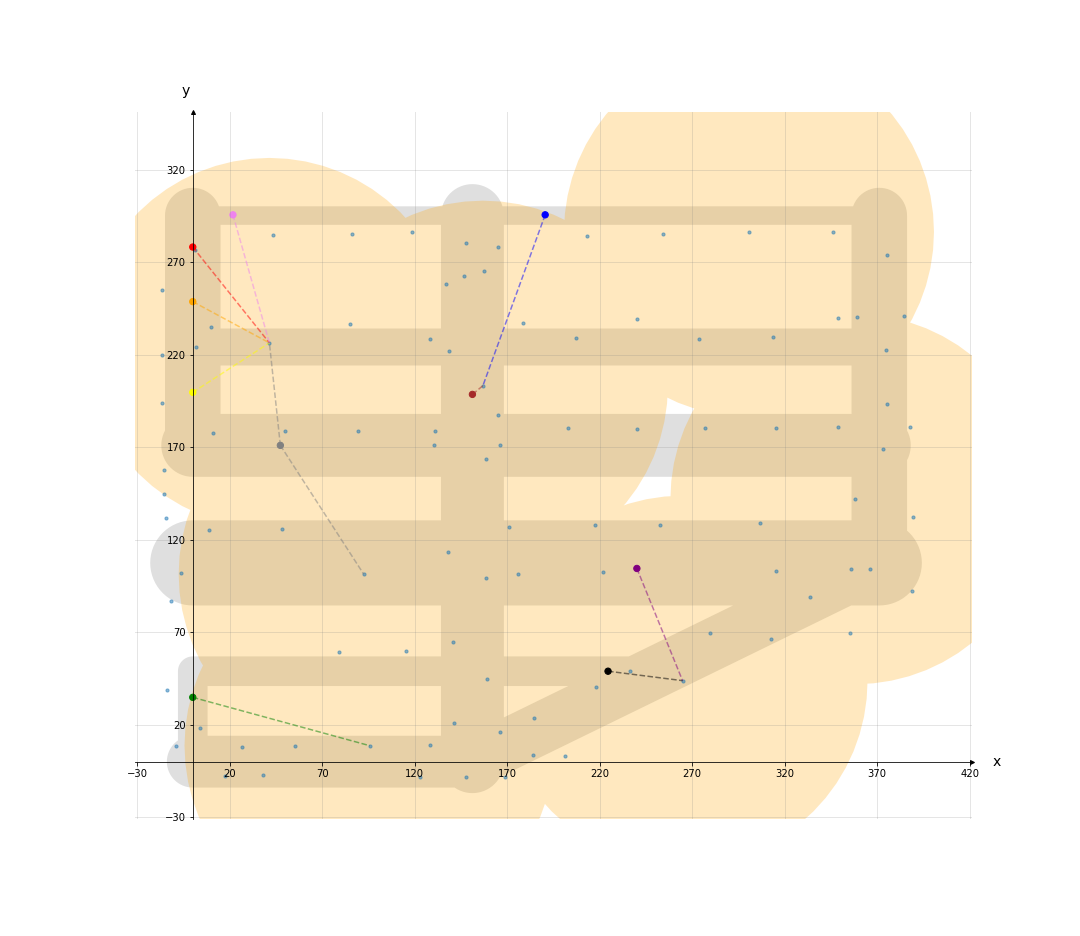
\includegraphics[width=14cm]{1.png}
			
			\small \textit{Fig. 1 Relationship between the basic factors}			
		\end{center}
	
		In this model, we actually need to have some detailed information about the whole transportation system in the area. In addition, we need to know about the driving pattern of the cars to make further discoveries about the autonomous driving system. In Fig. 1, we can clearly discover the relationship between the car, the lamppost and the cloud server.
		
		So the problem is divided into 3 main parts:
		\begin{itemize}
			\item Build a framework for evaluating the smart lamppost modification plans based on cost and coverage of the road by the sensor and the WiFi communication.
			\item Give a plan for smart lamppost modification in an area of any city according to the data given.\cite{Map}
			\item Evaluate the lamppost modification plan based on our model and find the strengths and weaknesses of our model.
		\end{itemize}
		\subsection{General Assumptions}
		\begin{itemize}
			\item \textbf{All the cars have the same scale.}
			
			\textit{We assume that all the cars can be seen as a car which is 4.8m in length and 1.6m in width. This can flatten the neighborhood which we take into consideration.}
			\item \textbf{The impact of buildings is not taken into consideration.}
			
			\textit{Since the distance between two roads is far from the detection zone, the buildings will not affect the detection of the road.}
			\item \textbf{Vehicles drive on the left side according to the standard of Hong Kong.}
			\item \textbf{Neighborhood intersection is not taken into consideration.}
			\item \textbf{Most of the calculation is completed on the client side.}
			
			\textit{There are different types of car on the road. Since the cloud side can't afford such large amount of calculation, we assume that the most of it is completed on the client side.}
			\item \textbf{The information that the cars need is of the same number at any time of the process.}
			
			\textit{In our dynamic model, the amount of information that each car requires is assumed to be a constant, which, in real life, varies according to the inherent attributions of the car. }
		\end{itemize}
	
	\newpage
	\section{Model 1: Evaluation Model}	
		\subsection{Model Overview}
		In this model, we will establish an indicator framework for the purpose of evaluating smart lamppost modification plans. By comparing the weight of different road types according to the cars' speed, acceleration, deceleration and reaction, we can clearly get the relationships of these areas. Basic road types include normal roads and crossroads. In this model, crossroads is defined as a circle with a radius of 50m, centering at the middle of the crossing.
		\begin{center}
			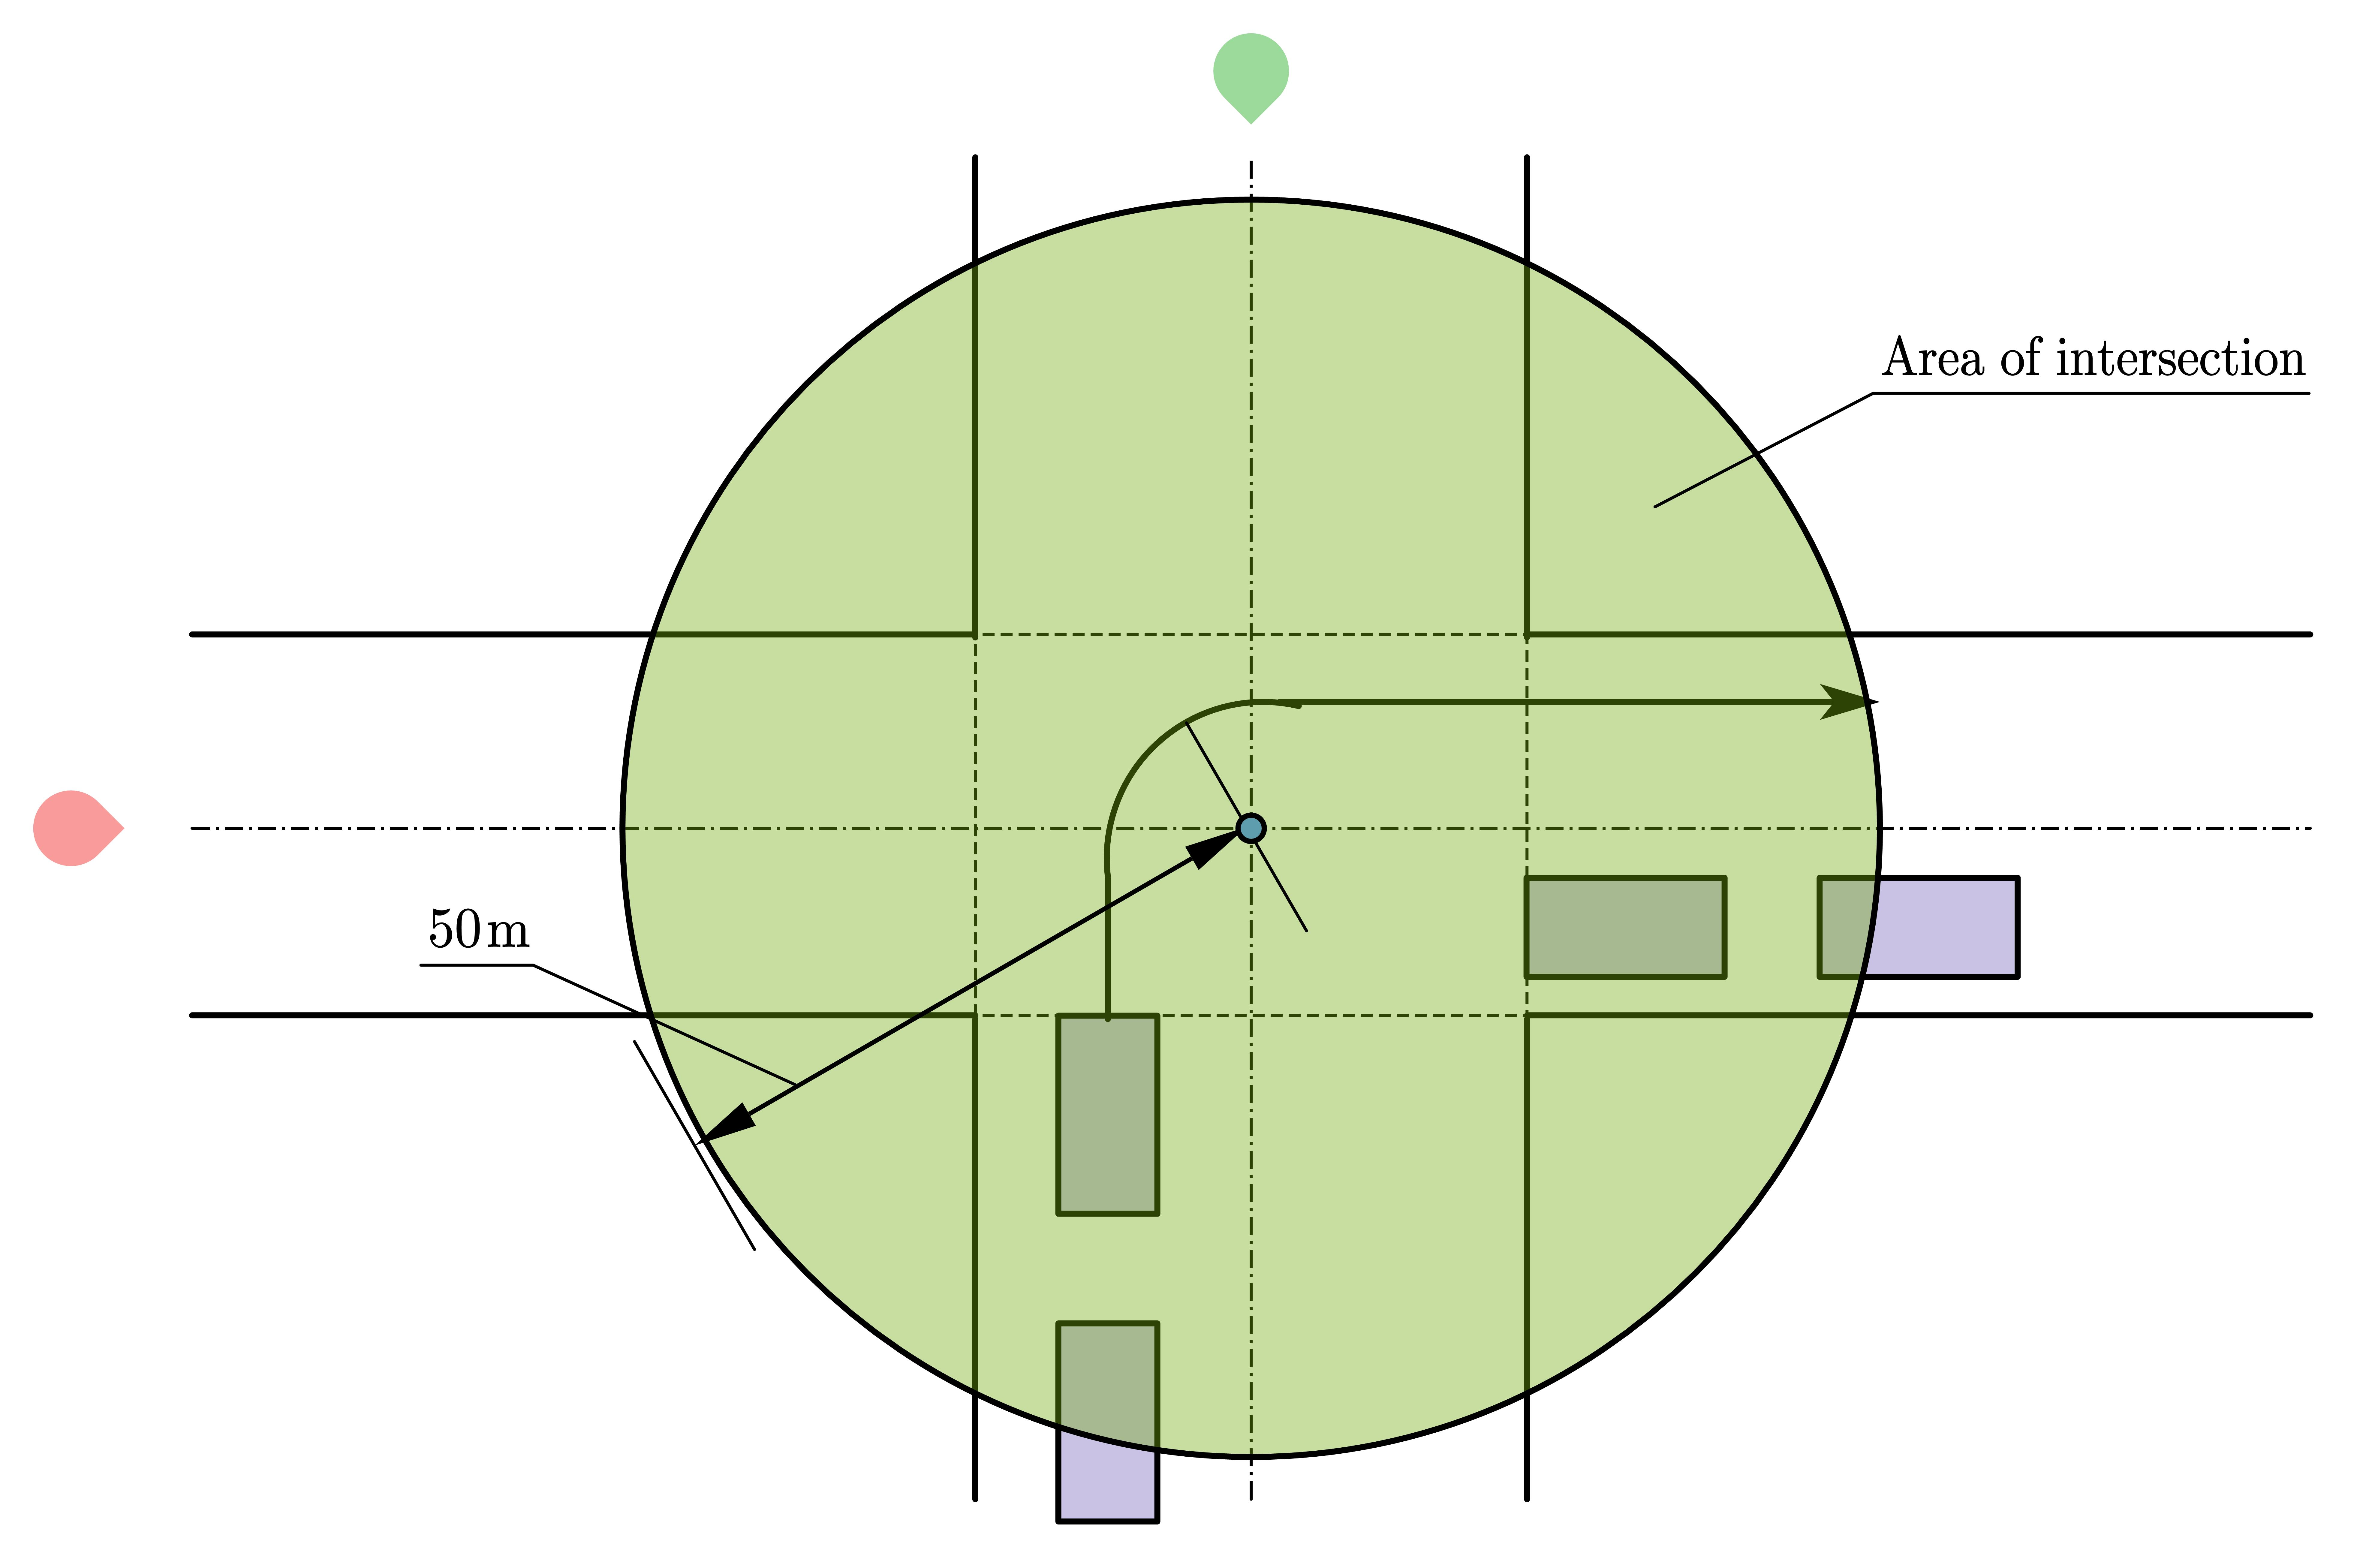
\includegraphics[width=7cm]{stimulation.jpg}
			
			\small \textit{Fig. 2 Driving Pattern in Crossroads}
		\end{center}
		\subsection{Assumptions}
		\begin{itemize}
			\item \textbf{All the destinations can be detected and can be abstracted as a dot.}
			
			\textit{To flatten the driving routine, we assume that all the destinations are only dots. When the car which has the shape of a car reach its destination, it will disappear immediately.}
			\item \textbf{The car will update its newest driving data at any time of the driving process.}
			
			\textit{To make sure that we can supervise the driving process and the location of cars connected to LiDAR and WiFi, we assume that the data will be updated at any time of the day.} 
		\end{itemize}
		\subsection{Variables and Constants}
		\begin{tabular}{ll}
		\hline
		Symbol&Definition\\
		\hline
		$S$&Evaluating Index\\
		$P$&Overall Cost\\
		$a_1$&The Coverage Rate of Sensors on Crossroads\\
		$a_2$&The Coverage Rate of Sensors on Normal Roads\\
		$b_1$&The Coverage Rate of WiFi Communication on Crossroads\\
		$b_2$&The Coverage Rate of WiFi Communication on Normal Roads\\
		$k_1$&Weight of Crossroads\\
		$k_2$&Weight of Normal Roads\\
		$b$&The rate of the most cars that can be connected to WiFi\\
		$k_3$&Weight of $b$\\
		\hline
		\end{tabular}	
		\subsection{Determining the Factors}
		In this model, we focus on the coverage rate of LiDAR and WiFi on different road type. For example, we describe $a_1$ as $\dfrac{S_\text{Coverage of Sensors on Crossroads}}{S_\text{all}}$. In the same way can we define $a_2$, $b_1$, $b_2$.
		
		When an autonomous driving cars are driving, the passengers inside usually thinks more about their safety when passing crossroads. This shows that the crossroads are more important than normal roads in our framework, so we can infer that:
		$k_1 \gg k_2$
		
		Therefore by defining the weight of coverage rate in different areas, we find out a simple formula describing the effectiveness of the system:
		$$S=\dfrac{k_1(a_1+b_1)^3+k_2(a_2+b_2)+k_3b}{P}$$
		$$(k_1>k_3>k_2)$$
		
	
	\newpage
	\section{Model 2: Modification Plan}
		\subsection{Model Overview}
		Now that we have established a basic framework of evaluating modification plans, we need to make sure that a plan can indeed be carried out in any selected city which have the economic ability to realize autonomous driving systems.	In this model, we will focus on the smart lamppost modification plan based on the transportation system in Wanzai Area,iHong Kong.\cite{Map} (See Appendix) We can abstract this map into a rectangular coordinate system. In Fig. 3, the red line refers to the road in this area and the blue dots refers to the lampposts that can be installed with LiDAR sensors and WiFi Access Points. Having this map, we can easily demonstrate the effect of smart lampposts on nearby cars.
		\begin{center}
			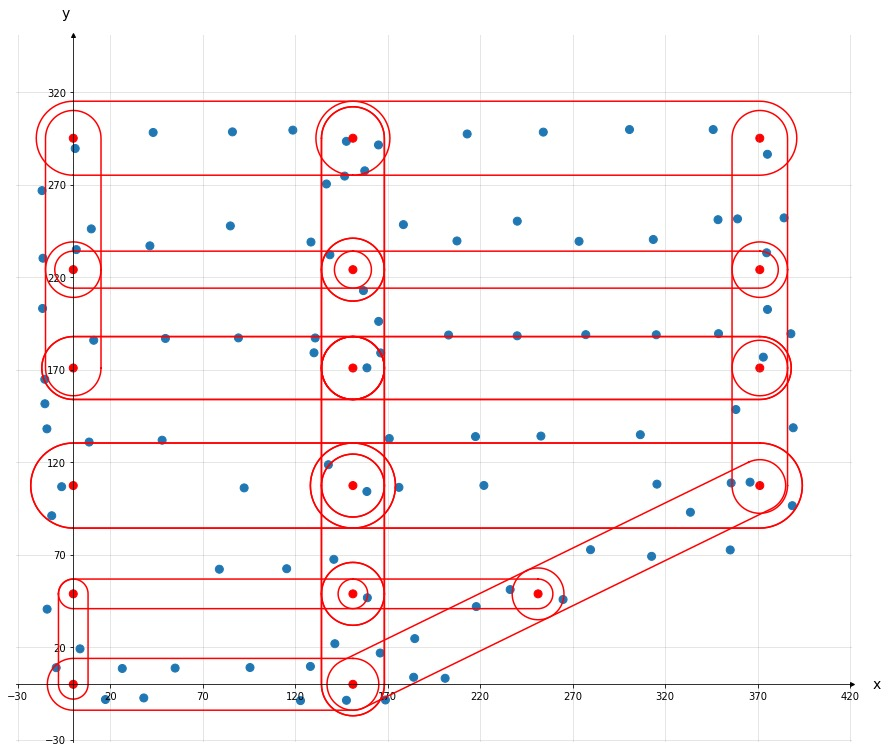
\includegraphics[width=8cm]{abstract.jpg}
			
			\small \textit{Fig. 3 Map of Wanzai Area}
		\end{center}
	
		\subsection{Definition and Assumptions}
		Based on the traffic rules and the geographic conditions in Wanzai Area, we make the following assumptions.
		\begin{compactenum}[1, ]
		\item We assume that an autonomous driving need no time to turn left and 5 seconds to turn right. The number comes from the calculation according to the average width of roads and the highest speed to change direction safely in normal conditions. This means that when a car turn right, it will disappear immediately and appear at the end of the line in this road 5 seconds later. In this process, the car will exert no impact neither on other cars nor on the queuing line.
		\item After searching the traffic rules in this area, we find that Gaoshida Avenue has a speed limit of 70km/h (19.5m/s) and other roads have a speed limit of 50km/h (14.0m/s). To make sure that our model is safe and can fit the traffic rules, we assume that all the cars drive on normal roads at a constant speed of 50km/h (14.0m/s).
		\item For we mainly focus on the driving condition of cars and their relationship with the smart lampposts, pedestrians are ignored in this model.		
		\item Through our calculation, the stopping distance turns out to be at least 16m. To ensure that our plan can make whole use of the technology, we need to make sure that LiDAR can cover all the crossroads.
		\item Because a single WiFi Access Point can only get connected to 4 cars at a time, we need to consider the cars which are not connected to WiFi technology. Now we assume that the cars drive a  constant speed and will get connected to WiFi as soon as the last car leaves the area.
		\end{compactenum}
		So now let we assume that we are in an autonomous driving car. If the car is running normally, it will drive at a constant speed when on normal roads. When it receives the information provided by WiFi technology, then it will estimate whether it's turning or driving, whether it's going to meet red lights and when it's going to change its direction.
		

	
		\subsection{Model Calculation}
		To get further understanding of the transportation system in this area, we use Q-learning to summarize our way of distributing and find out the best modification plan.
		
		Q-learning\cite{Qlearning} is an off policy reinforcement learning algorithm that seeks to find the best action to take given the current state. It doesn't need any policies because the Q-learning function learns from actions that are outside the current policy by taking different actions randomly. More specifically, Q-learning seeks to learn a policy that maximizes the total reward. Therefore, we can use Q-learning to find the location of smart lampposts installed with WiFi and LiDAR technology that best fits the condition in the selected area.
		\subsection{Variables and Calculations}
		\begin{center}
		\begin{tabular}{ll}
			\hline
			Symbol&Definition\\
			\hline
			r&Road type\\
			d&device\\
			$L_1$&Lampposts with only LiDAR\\
			$L_2$&Lampposts with only WiFi\\
			$L_3$&Lampposts with both\\
			\hline
		\end{tabular}
		\end{center}
	\begin{algorithm}
		\caption{Find the best modification plan.}
		\label{Type}
		\begin{algorithmic}
		\STATE \textbf{def} Get\_State(Distribution)
		\STATE Cost = $5000\cdot L_1+3000\cdot  L_2+10000\cdot L_3 $
		\STATE \textcolor{red}{\# Formula of calculating coverage: $\dfrac{S_{\mathrm{road\ covered}}}{S_{\mathrm{roads}}}$​​}
		\STATE 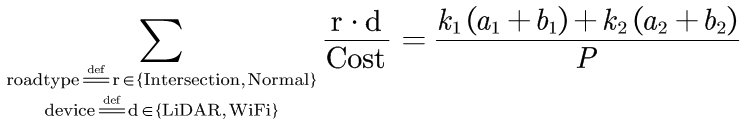
\includegraphics[scale=0.6]{formula.jpg}
		\STATE \textbf{return} State
		\STATE \textbf{end def}
		\STATE L = Set of all SmartLamps
		\STATE done = \textbf{\textcolor{violet}{False}}
		\STATE initialize q\_table, LEARNING\_RATE and DISCOUNT
		\WHILE{not done}
		\STATE update q\_table
		\ENDWHILE
		\FOR{lamp in L}
		\WHILE{in attempt to change the configuration of lamp}
		\IF{Get\_State(new\_distribution) > Get\_State(current\_distribution)}
		\STATE change distribution
		\ELSE
		\STATE remain
		\ENDIF
		\ENDWHILE
		\ENDFOR
		\STATE previous loop $\rightarrow$ find q\_table[max\_distribution] and corresponding action
		\STATE current\_distribution = q\_table[current\_state + action]
		\STATE new\_distribution = (1 - LEARNING\_RATE) * current\_distribution +\\ LEARNING\_RATE$\times$ ($\Delta$ Get\_State + DISCOUNT * max\_distribution)
		\STATE q\_table[current\_state + action] = new\_distribution
		\STATE conduct the loop continuously until the previous loop doesn't alter anything:
		\STATE done = \textbf{\textcolor{violet}{True}}
		\end{algorithmic}
	\end{algorithm}

	\newpage
	\subsection{Result}
	According to these rules and the calculation ideas we have put foward, we finally drew a complete figure of our plan, which is shown in the Fig. 4 below.
	\begin{center}
		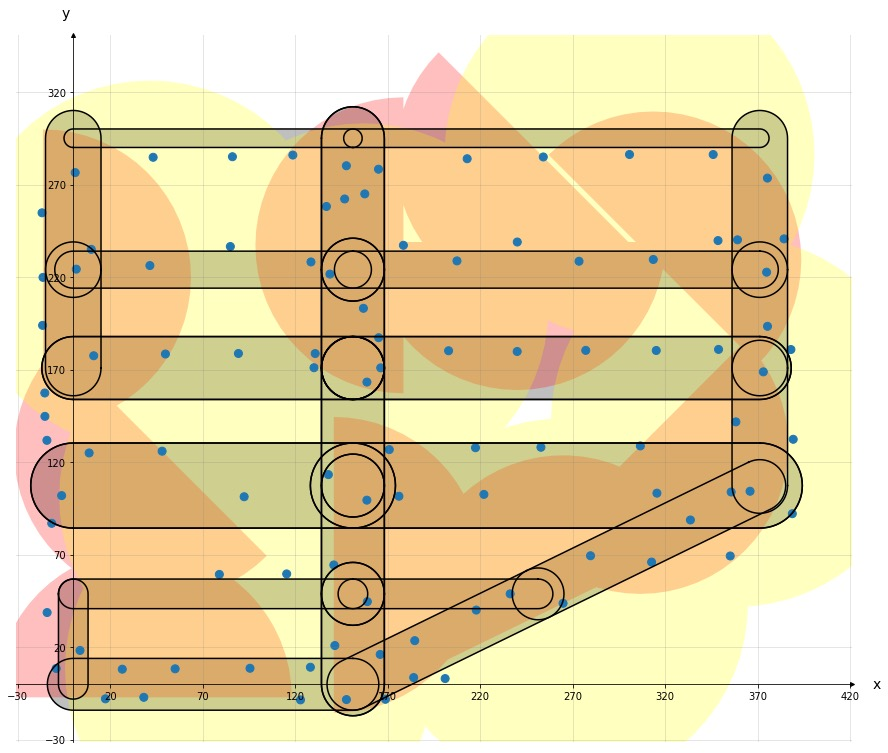
\includegraphics[width=10cm]{final.jpg}
		
		\small\textit{Fig. 4 Final Result of Distribution}
	\end{center}

	In Fig. 4, the yellow part refers to the WiFi-covered area while the red part refers to the LiDAR-covered part. We can see that most of the space in this area is now covered by Wifi, so cars driving in this area can get connected to the cloud server and get the data provided to make better driving plans. Because WiFi technology has a wider range of coverage than LiDAR technology, there are parts which are WiFi-covered but not LiDAR-covered. But since we have assumed that cars drive at a constant speed when they're not LiDAR-covered part, the impact can be ignored.
	
	In all we need to distribute 16 smart lampposts. There are 9 lampposts which only need to be installed with LiDAR sensors, 6 lampposts which only need to be installed with WiFi access points and only 1 lamppost to be installed with both of them. There position coordinates are shown in the two charts below.
\newpage
\begin{center}
	\textit{Table 1: LiDAR Lamppost Coordinates}
	
	\begin{tabular}{||r|r|r|r||} 
		\hline
		& xLiDAR & yLiDAR & Angle\\
		\hline
		1 & 48.0341 & 126.007 & 135\\
		2 & -16.3686 & 219.959 & 270\\
		3 & 140.853 & 64.5057 & 270\\
		4 & 178.457 & 237.312 & 90\\
		5 & 240.017 & 239.083 & 180\\
		6 & 313.536 & 229.637 & 315\\
		7 & 306.539 & 128.857 & 225\\
		8 & 38.1314 & -7.04044 & 0\\
		9 & 254.081 & 285.061 & 135\\
		10 & 264.77 & 43.785 & 26\\
		\hline
	\end{tabular}
\end{center}

\begin{center}
	\textit{Table 2: WiFi Lamppost Coordinates}
	
	\begin{tabular}{||r|r|r||} 
		\hline
		& xWiFi & yWiFi\\
		\hline
		1 & 41.427 & 226.357\\
		2 & 92.3732 & 101.392\\
		3 & 95.542 & 8.66328\\
		4 & 156.851 & 203.248\\
		5 & 264.77 & 43.785\\
		6 & 300.676 & 286.392\\
		7 & 358.18 & 141.86\\
		\hline
	\end{tabular}
\end{center}

	After calculating the cost, we find that we only need to spend \$73000 on our smart lamppost modification plan. 
	\subsection{Sensitivity Analysis}
	In this part, we will discuss the sensitivity of our plan and find out whether our plan is useful enough for the city and everyday transportation.
	
	After calculation, we get the formula describing the sensitivity of our model.
	$$I_{sensitivity}=\dfrac{\dfrac{\Delta \mathrm{U}}{\mathrm{U}}}{\dfrac{\Delta S}{S}}$$
	
	As mentioned in the modification plan,  we get a detailed picture of the area we study and the position of each lamppost we need to distribute. By changing the position coordinates of LiDAR sensors and WiFi Access Point randomly, we can see the change of variables mentioned in Evaluation Model. Later we get rid of some abnormal data and calculate the variance of our data: 16.7357874. 

	In this formula, $U$ refers to the uniformity of this model.To express the distribution of smart lampposts in a mathematical way, we used the “distribution index” $U$ which is defined as following:\cite{Sensitivity}
	
	$$U = \frac{\overline{d_\text{min}}}{\text{R}} = \frac{\left(\text{the }\text{n} \text{ minimums of the }\frac{n(n-1)}{2} \text{ distances between } \text{n} \text{ lampposts } /n \right)}{2 \cdot \sqrt{area \cdot n^{-1} \cdot \pi^{-1}}}$$	
	\begin{center}
	(In this model, $n$ refers to the number of the lampposts. )
	\end{center}

	In theory, $U$ is a real between 0 and 1. When the $U$ is bigger, the distribution is more average.
	\begin{center}
		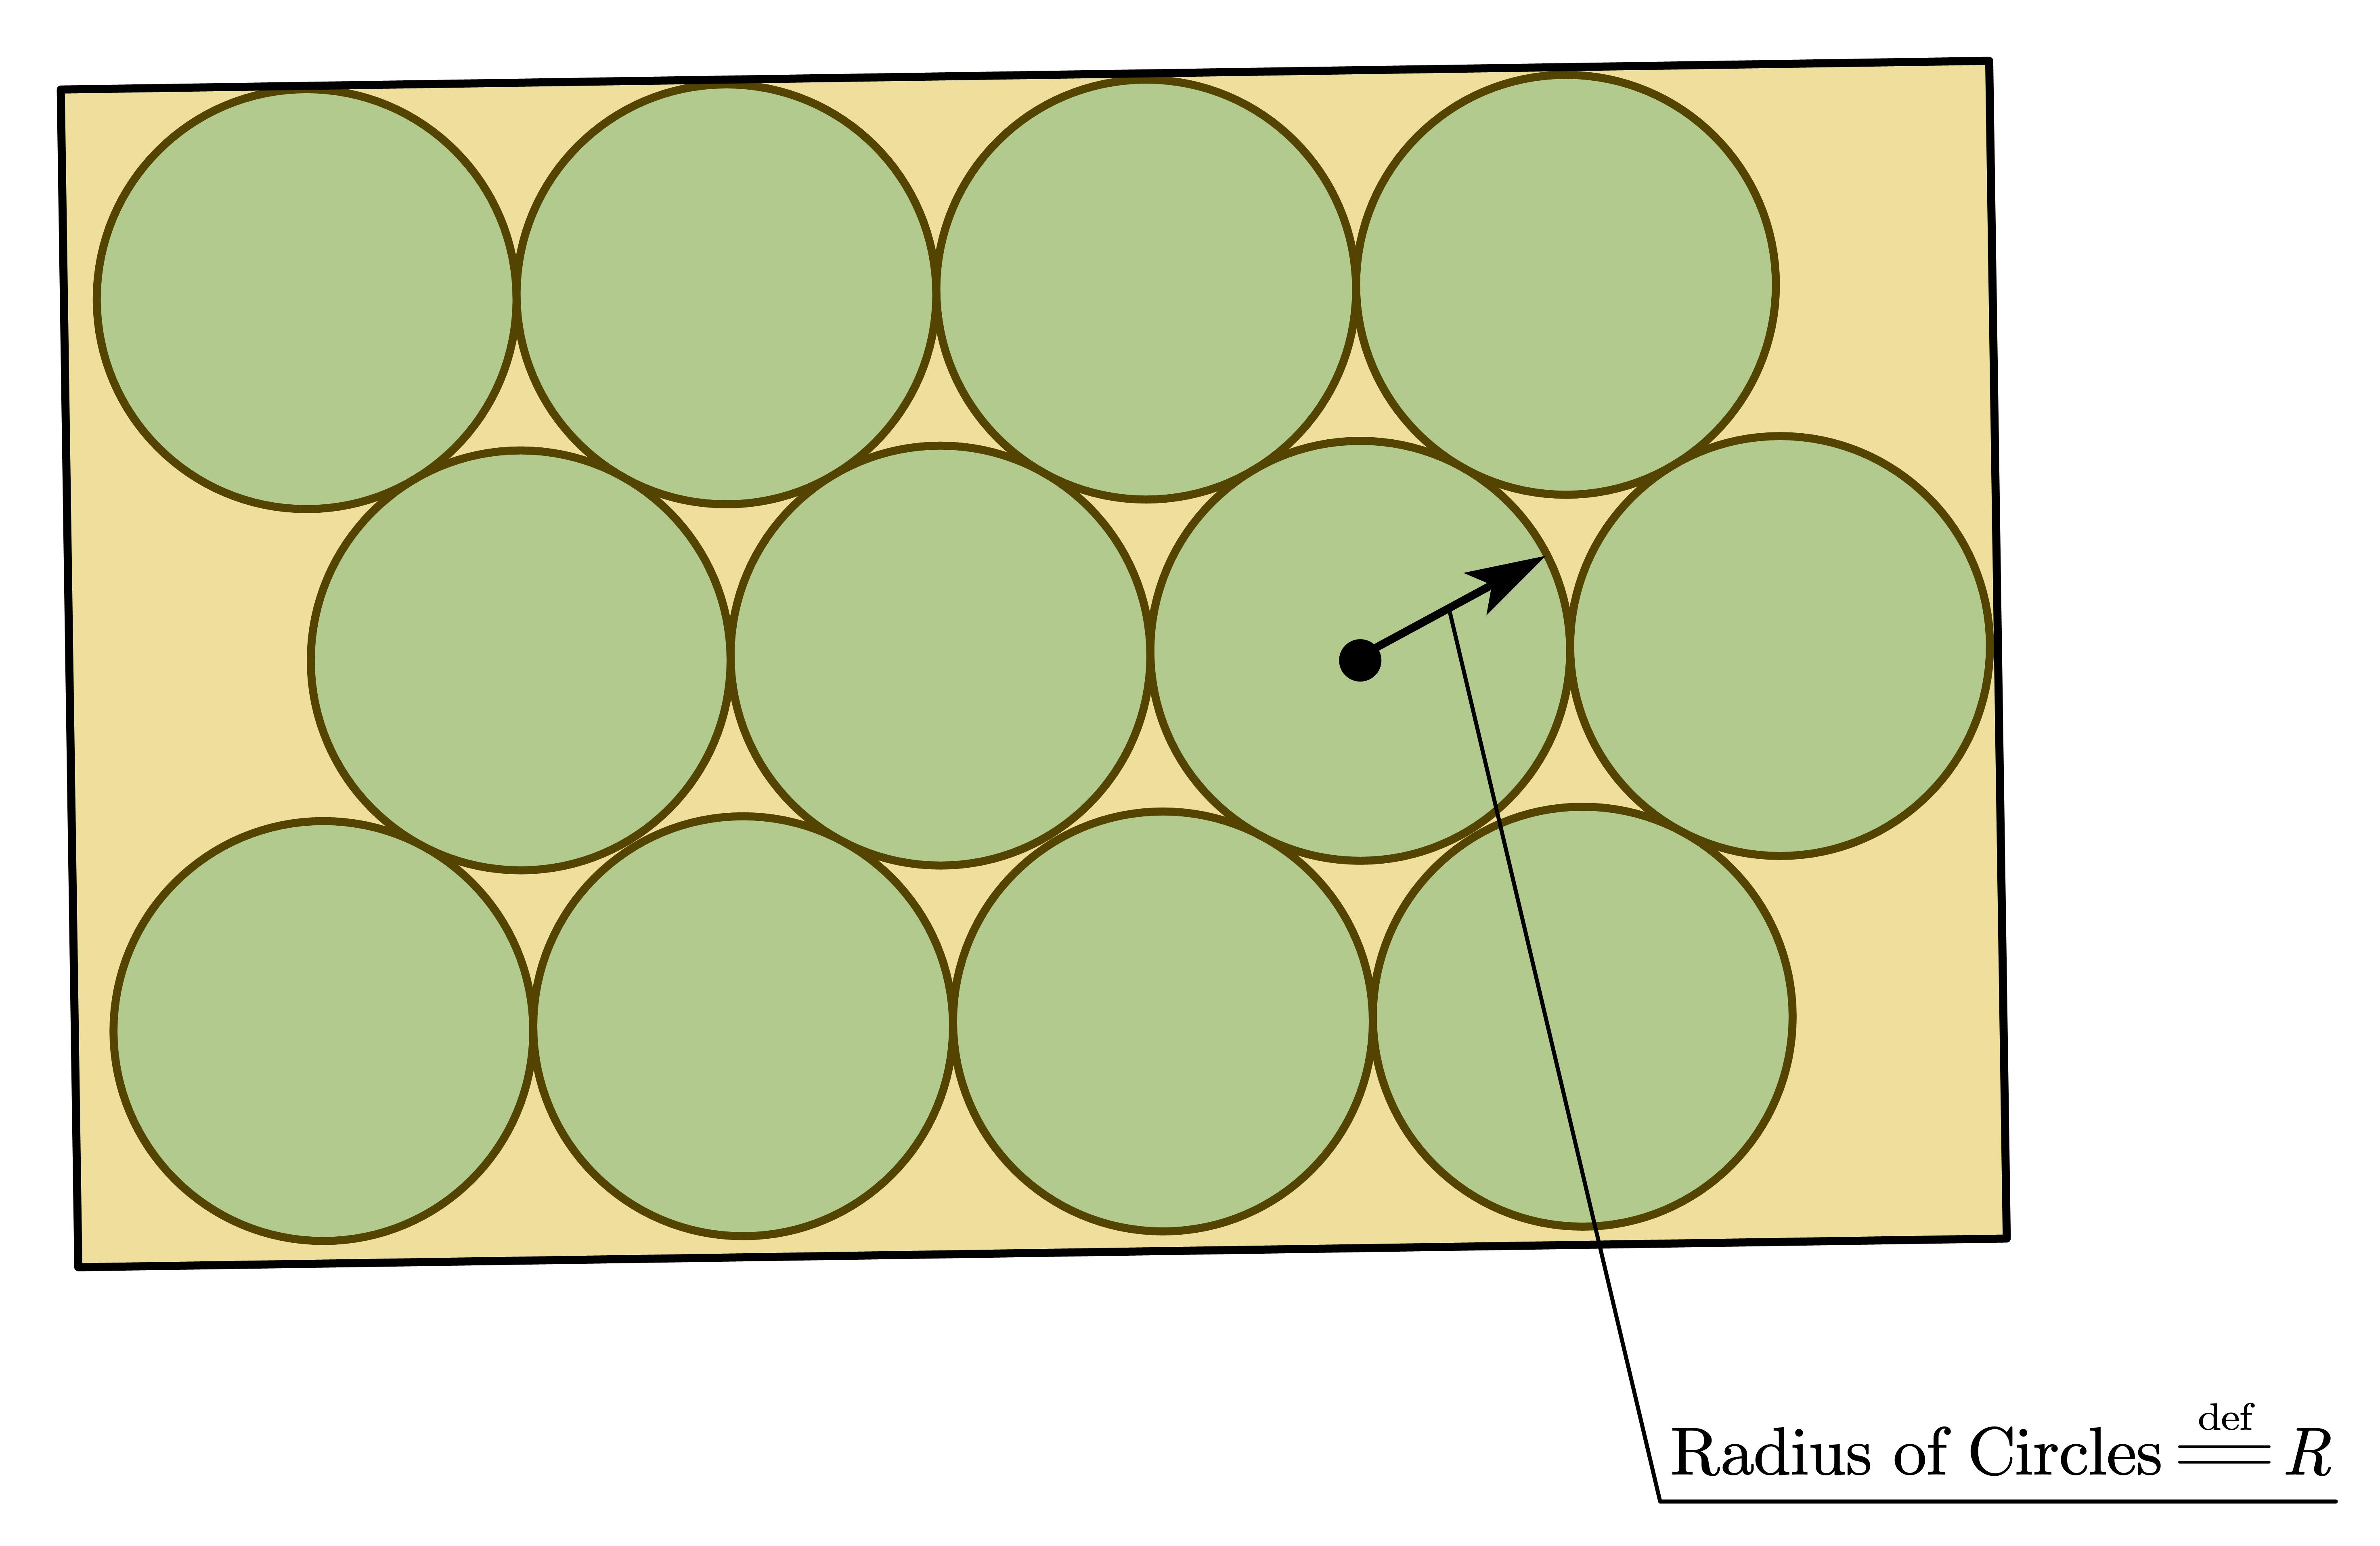
\includegraphics[width=8cm]{uniformity.jpg}
		
		\small \textit{Fig. 5  Describing Uniformity}
	\end{center}
	
	Finally we get the number of $U$ in our model: 4.0065.
	This is a reasonable number and it shows that our model is robust and reasonable. It can apply to various changes and can make better distribution plans.
		
		
	
	
	\newpage
	\section{Evaluation of Our Own Plan}
	\subsection{Problem Overview}
		In the last section, we have analyzed the sensitivity of our plan. In this part, we will calculate the coverage area and the coverage rate of our plan accurately. Later, we use our index to evaluate our plan. By getting the number and comparing it with other plans in which some variables are changed randomly, we will find the strengths and weaknesses of our plan. Later we will show what improvements we decide to make to our model and what we can do with the development of the automatic driving system. A dynamic model is developed to solve the problem of inaccurate evaluation.
	\subsection{Calculation of the Evaluation Index}
	We calculate the evaluation index of different conditions as we change the location coordinates of lampposts and the angle of LiDAR sensors to find the rise and fall of its effectiveness which is shown by the evaluation index. 
	
	After calculation, we find out that the evaluation index of our plan is 0.7233. However, after changing the factors, the number ranges from 0.54 to 0.71. This shows that our model has great effectiveness and can best fit the traffic system in Hong Kong now. Also, we discover that the change in WiFi location will let the number have a sharper decrease, so we can infer that WiFi location will pose a greater impact on the modification system. If we want to make further improvement, we can focus on the change in WiFi distribution.
	
	\subsection{Verify Our Model}
		To make sure that our model can apply to everyday traffic routine, we use C++ to simulate the driving process and calculate the connection rate of WiFi.
	
		​	In the simulation process, we consider each road block as an array of cars. In each round of the update process, we begin the operation of each road from the first car in its array till 	the last. Notice that in our dynamic updating process, each car, except from the first in the array, possesses a unique action dependent on its predecessor. In short, the car evaluates its capability of reaching the next intersection before the red light and performs correspondent deceleration or acceleration while controlling the safe distance between the two cars at the same time, the mathematical formulas of which are shown in the code below. As for the first car in the array, it similarly decides its action, and randomly decides to turn to the next road if it ultimately reaches the intersection with the green light on.
		
	    Secondly, we use bipartite graphs to simulate the connection process of WiFi.When calculating the rate of cars connected into the WiFi system ($b$), we can use an algorithm which matches WiFi lamps with cars to find how many cars can be connected into the WiFi system.
		
	
	
	\begin{algorithm}
		\caption{Simulation of the driving condition.}
		\label{type}
		\begin{algorithmic}
			\STATE \textbf{def} update(test):
			\STATE time += 0.5 \textcolor{red}{\# updating once every half a second}
			\FOR {k in cars \textcolor{red}{\# run through all the cars}}
			\IF {car No. k is going to start turning at this time}
			\STATE pick a random direction at its crossroad for the car to go to
			\STATE decide the time the car spends on this turning (depending on the direction of the turning)
			\ENDIF
			\IF {car No.k is already turning at this time}
			\STATE it continues turning regardless of traffic lights
			\ELSE
			\STATE \textcolor{red}{\# car No.k is in the middle of a road}
			\STATE calculate the location of this car at this time
			\STATE find the coming traffic light
			\IF {this car cannot pass the traffic light}
			\STATE calculate the minimum deceleration distance according to the original  speed of the car and its maximum deceleration rate
			\IF {the distance between the car and the light is no longer than this distance}
			\STATE it decelerates in its maximum decelerate rate
			\ELSE
			\STATE calculates its maximum speed and then accelerate to this speed in the maximum acceleration rate and then decelerate its speed to 0 (and just stops at the red light)
			\ENDIF
			\ELSE
			\IF {the distance between the car and the traffic light is no longer than the distance the car goes in half a second}
			\STATE \textcolor{red}{\# it will turn in the coming half second}
			\STATE label it as it would turn in the next half a second
			\ENDIF
			\ENDIF
			\ENDIF
			\ENDFOR
			\STATE \textbf{end def}
		\end{algorithmic}
	\end{algorithm}


	
	\newpage
	\subsection{Result Analysis}
	\subsubsection*{Strength}
	\begin{itemize}
		\item \textbf{Our model has strong flexibility.}
		
		Our models are generic.Except from the necessary road map data, our model completely depends on the internal algorithms of the system, thus it can be applied to various conditions.
		\item \textbf{Efficiency}
		
		In model 2 we modified the highly-efficient Q-learning algorithm, which quickly narrows the range until it gets the optimal result.
	\end{itemize}
	
	\subsubsection*{Weaknesses and Expectation}
	\begin{itemize}
		\item \textbf{We have limitation when facing discretization of variables.}
		
		The standard Q-learning algorithm applies only to discrete action and state processes. When there are less than 30 lampposts, it can no longer find the best data largely due to the cause of dimenssionality.\cite{drawback}
				
		\item \textbf{There is difference between our model and reality.}
		
		Nowadays, the WiFi technology is not so efficient and the calculation on the client side doesn't have such a speed as assumed in our model. Our model should make improvements. In addition, we should always pay attention to new technology as the technology is developing fast.
	\end{itemize}
	\section{Model 3: Improved Model}
	\subsection{Model Overview}
		When analyzing the strengths and weakness of our model, we mentioned that we do not have a dynamic model to make our calculations more accurate. Now, we try to make it more accurate by using C++.
	\subsection{Assumptions}
	\begin{itemize}
		\item \textbf{$\forall L, V_{M,L}\xlongequal{\mathrm{always}}50\mathrm{km}/\mathrm{h}$}
		
		\textit{By searching for data on websites\cite{Traffic}, we found out that all roads of such scale in our model have a speed limit of $50\mathrm{km}/\mathrm{h}$, for given the fact that only the bottom of Gloucester Road is connected with the rest of the map.}
		\item \textbf{The car inflow and outflow of the selected area is always at an equilibrium.}
		
		\textit{Or else, $N_{C,L}$​​​​​​ is either consistently decreasing or increasing, which, given the isolation and the areal limitations of the model, is apparently unreasonable.}
	\end{itemize}
	\subsection{Notation}
	\begin{tabular}{ll}
	\hline
	Symbol&Definition\\
	\hline
	$\tau _{L_1\rightarrow L_2,R}​​$& the red-light interval of road $L_1$ at its intersection with road $L_2​$\\
	$\tau _{L_1\rightarrow L_2,G}​$& the green-light interval of road $L_1​$ at its intersection with road $L_2​​$\\
	$W_{L}​​$& the width of road L​\\
	$T_L​$& the duration of a total light period\\
	$V_{M,L}​​$& the maximum velocity of cars on road L​​\\
	$N_{C,L​}$& the number of cars on road L​\\
	\hline
	\end{tabular}
	\subsection{Materializing the Traffic}
	Firstly, we set up several functions concerning cars, roads, and traffic lights using C++. As for the dynamic process, the real-time performance of cars is simulated
	Because all the roads are of approximately the same width, deriving the equation above the first assumption, we can get the following relationship:
	
	$$\forall I,T_{I,turn}=\begin{cases}
		0.5,turn=\mathrm{left}\\
		1.5,turn=\mathrm{straight}\\
		5,turn=\text{right or turn around}\\
	\end{cases}$$

	\begin{align}
		\dfrac{\tau _{L_1\rightarrow L_2,G}}{\tau _{L_2\rightarrow L_1,G}} &\propto \dfrac{W_{L_1}}{W_{L_2}}\\
		\forall L_1, L_2​ \text{ as lights, } \tau _{L_1\rightarrow L_2,G}+\tau _{L_1\rightarrow L_2,R} &\xlongequal{\mathrm{always}} T_L
	\end{align}

	In this relationship, (5.2) apparently maintains the numerical proportion of traffic light intervals as shown in (5.1), and it is also beneficial to our discrete model, since the timelines of different traffic lights can be easily synchronized.
	
	In our model, we assume that the time of cycle of red lights and green lights is 100 seconds in total. In addition, we introduced the concept of 'yellow lights' so as to offset the inaccuracy of updating the model discretely: a certain time is given for each vehicle to either decelerate or accelerate at its maximum. 
	
	When it comes to deceleration, we have the constants and variables below
	\begin{center}
	\begin{tabular}{ll}
		\hline
		Symbol&Definition\\
		\hline
		$v_0$&Initial Velocity\\
		$a$&Acceleration\\
		$x$&Minimum Braking Displacement\\
		$t$&Time\\
		$\theta$&the Angle of the Direction of the Car's Displacement and Horizontal Direction\\
		$l$&Displacement\\
		$v$&Velocity\\
		\hline
	\end{tabular}
	\end{center}
	
	So we can get the minimum breaking displacement is:
	$$x=\frac{v^2}{2a}$$
	If $a$ refers to the largest acceleration, the displacement in that period is:
	\begin{align*}
	\mathrm{d}v &=a\mathrm{d}t\\
	\mathrm{d}l &=v\mathrm{d}t
	\end{align*}
	So we can infer that:
	\begin{align*}
	 \Delta x &= l\sin \theta\\
	 \Delta y &= l\cos \theta.
	\end{align*}

	Secondly, for different states of the output of the dynamic model, we use the Hungarian algorithm to get the optimal connection scheme of cars and tests whether it is optimal. The process is shown in the algorithm below.
	
	We construct a bipartite graph G($V_14$ ,$V_2$;E)​, where $V_1$ refers to the set of lampposts, and $V_2$ refers to the set of all on-road vehicles. 
	$$\forall u\in V_1,v\in V_2, uv\in E\Leftrightarrow \text{the distance between u and v < 100m}$$
		\begin{algorithm}
		\caption{Match lampposts with WiFi}
		\label{type}
		\begin{algorithmic}
			\STATE \textcolor{red}{\# We consider that each of WiFi lampposts has four WiFi spots, with each one connecting to one car.}
			\STATE lines[] \textcolor{red}{\# lines[i] refers to the spots that can be linked to the car No. i}
			\STATE used $\leftarrow$ [] \textcolor{red}{\# judging whether a WiFi spot can be used}
			\STATE match $\leftarrow$ [] \textcolor{red}{\# record the matching car of each WiFi spot}
			\def \update{find(car): \textcolor{red}{\# judge whether a car can be connected (Hungarian algorithm)}}
			\FOR{i in lines[car] \textcolor{red}{\# all the spots that can connect with this car}}
			\IF{used[car][i] is 0}
			\STATE used[car][i] $\leftarrow$ 1
			\IF{match[line[car][i]] is 0 or find(match[line[car][i]]) is 1:\textcolor{red}{ \# this spot is not connected or this position can be spared}}
			\STATE match[line[car][i]] $\leftarrow$ car \textcolor{red}{\# record the pair}
			\STATE \textbf{return} 1\textcolor{red}{ \# this car can be connected}
			\ENDIF
			\ENDIF
			\ENDFOR
			\STATE \textbf{return} 0 \textcolor{red}{\# all the available spots cannot connect the car}
			
			\WHILE{updating the information of the cars}
			\STATE set 4 spots for each WiFi lamp (each spot can link at most one car)
			\FOR{k in cars}
			\FOR{i in WiFi lamps}
			\IF{the distance between WiFi lamp i and car k is no more than 100m}
			\STATE link an edge between car k and the 4 spots of WiFi lamp i 
			\ENDIF
			\ENDFOR
			\ENDFOR
			\ENDWHILE
			\FOR {k in cars}
			\STATE ans$\leftarrow$ans + find(k) \textcolor{red}{\# whether car No.k can be connected}
			\ENDFOR
		\end{algorithmic}
	\end{algorithm}
	
	\newpage
	By getting the moving pattern of each car, we get the complete figure of this autonomous transportation system. The dots in different colors refer to moving patterns of different cars.
	\begin{center}
		\begin{tabular}{cc}
		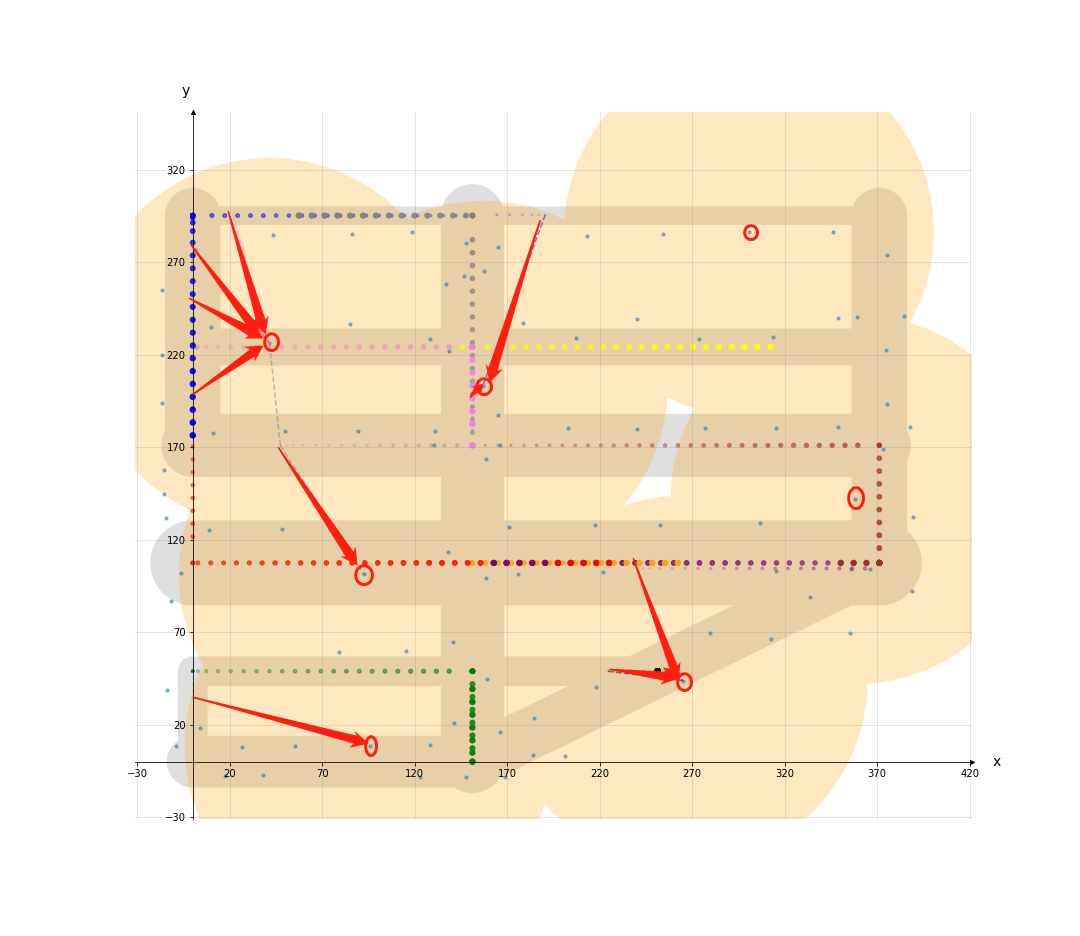
\includegraphics[height=6cm]{10.png}&	
		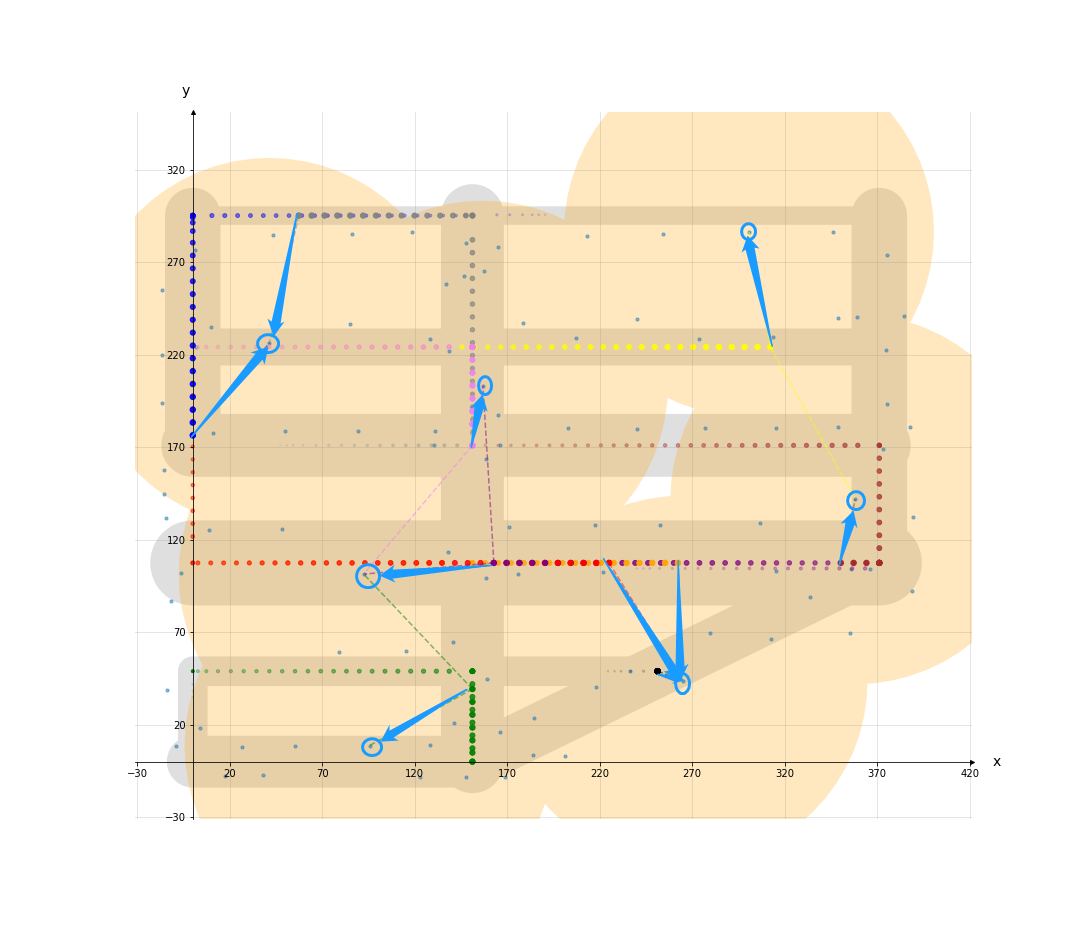
\includegraphics[height=6cm]{11.png}\\
		\small \textit{Fig. 6 $\quad t=0$}&
		\small \textit{Fig. 7 $\quad t=60$}\\
		\end{tabular}
		
		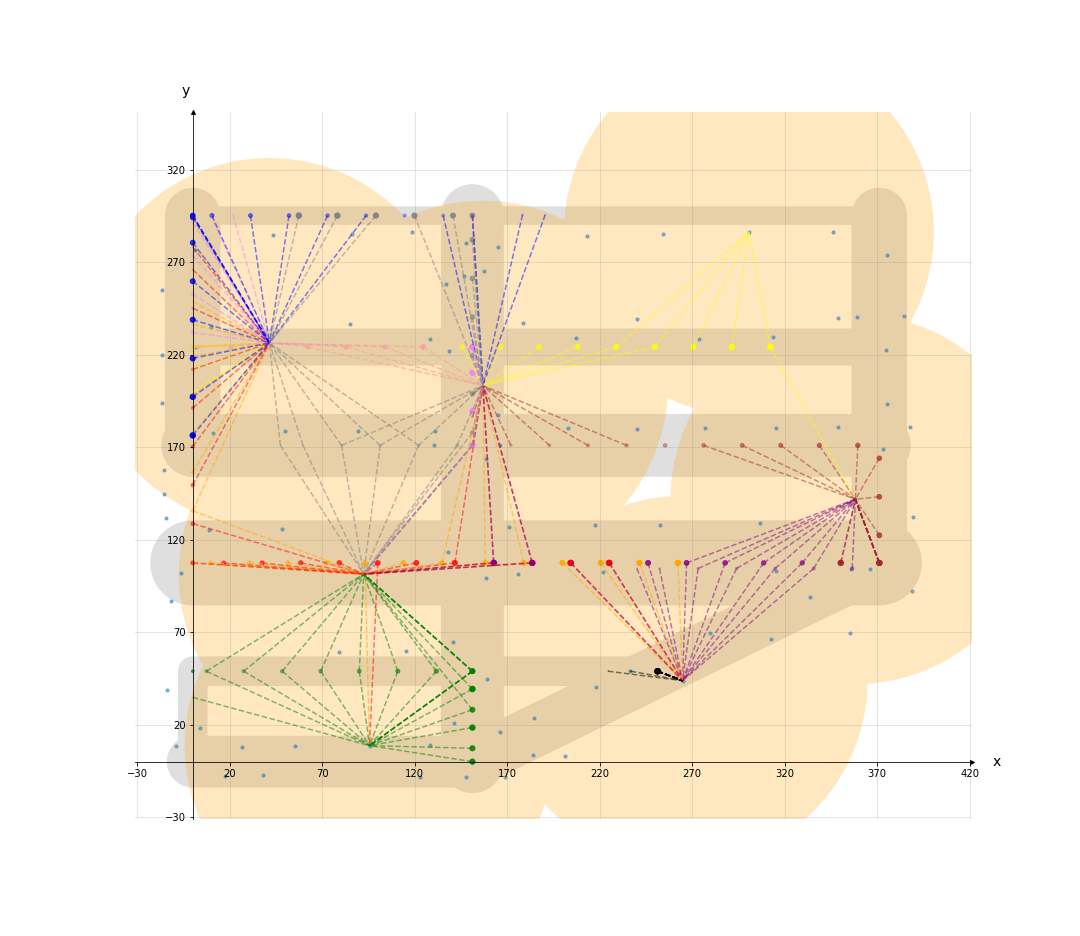
\includegraphics[width=10cm]{dynamic.png}
		
		\small \textit{Fig. 8 Describing the dynamic pattern.}
	\end{center}


	Finally, we manually optimize the installation under the conditions that meet the requirements which install the smallest set of all WiFi street light lines.
	
	Based on the Hungarian Algorithm, we can also make some improvements. The car which comes near to the crossroad will have a greater chance to get connected to the WiFi Access Point.
	\subsection{Strength and Weaknesses}
	\subsubsection*{Strengths}
	\begin{itemize}
		\item \textbf{Accuracy}
		
		Compared to Model 2, establishing a dynamic model adds realistic factors into the modification plan, such as red and green light. This will make our model more practical and more accurate. This is a great improvement based on the weaknesses of the last model.
		\item \textbf{Efficiency}
		
		In model 3, the intricate mechanism of the Hungarian algorithm helps us get the result within $\Theta \left( m+n \right)$, where $m$ and $n$ respectively refers to the number of vertexes and edges in the diagram.
	\end{itemize}
	\subsubsection*{Weaknesses}
	\begin{itemize}
		\item \textbf{Complexity}
		
		Because our algorithm is too complicated, it usually takes a lot of time to receive the correct data. Also, the algorithm is sometimes unstable.
		\item \textbf{Limitation in WiFi Technology}
		
		The maximum throughput of a WiFi Access Point is 800 Mbps.In our dynamic model, the amount of information that each car requires is assumed to be a constant, which, in real life, varies according to the inherent attributions of the car.  In this conception, the Hungarian algorithm will simply become a weighed two-dimensional optimization, optimizing car connection and information transferring at the same time. However, the model complexity and processing time will be greatly increased.
	\end{itemize}
	
	\newpage
	\thispagestyle{empty}
	\pagestyle{plain}
	\addcontentsline{toc}{section}{Appendix}
	\clearpage
	\section*{Appendix}
	\subsection*{Attachment 1}
	\begin{center}
		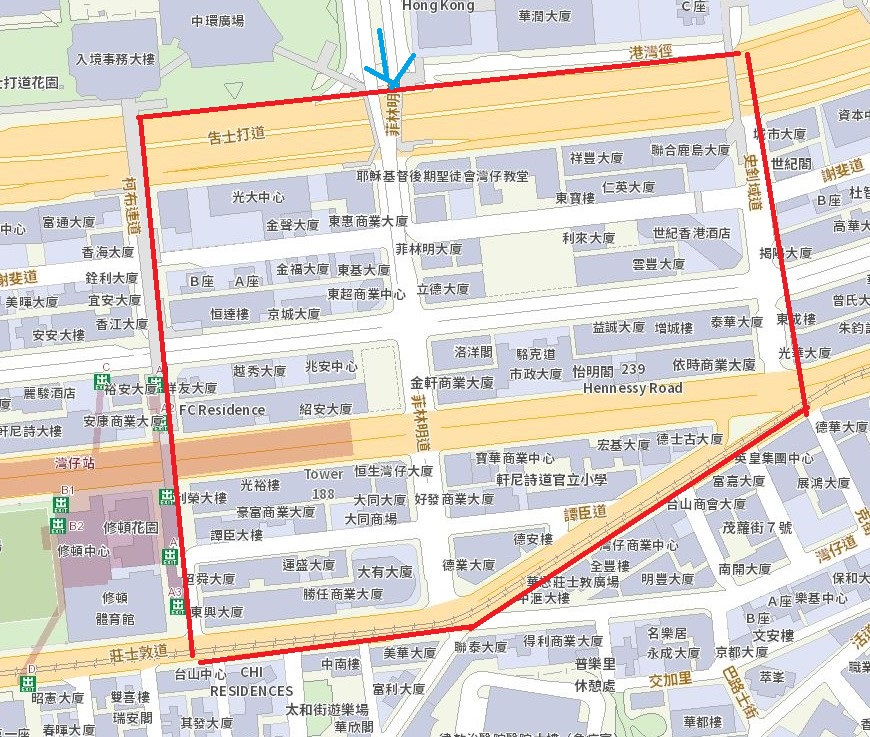
\includegraphics[angle=90,height=16cm]{map.jpg}
	\end{center}
	
	
	
	
	\newpage
	\thispagestyle{empty}
	% \setcounter{page}{\wholepages}
	\renewcommand\refname{References}
	\clearpage
	\addcontentsline{toc}{section}{References}
	\tolerance=500
	\begin{thebibliography}{100}
		\bibitem {Autonomous Driving Levels} Taxonomy and Definitions for Terms Related to Driving Automation Systems for On-Road Motor J3016\_201806, SAE International,\\ https://www.sae.org/standards/content/j3016\_201806/
		\bibitem {Map} Hong Kong Geographical Map, GEOINFO MAP,\\ https://www.map.gov.hk/gm/map/
		\bibitem {Sensitivity} Check if 2D points are evenly distributed, MathWorks MATLAB Answers John D'Errico,\\ https://www.mathworks.com/matlabcentral/answers/180860-check-if-2d-points-are-evenly-distributed
		\bibitem {Qlearning} Simple Reinforcement Learning: Q-learning, Andre Violante,\\ https://towardsdatascience.com/simple-reinforcement-learning-Q-learning-fcddc4b6fe56
		\bibitem {drawback} Q-learning, Wikipedia,\\ https://en.wikipedia.org/wiki/Q-learning
		\bibitem {Traffic} Speed Limits in Hong Kong, Wikipedia,\\https://en.wikipedia.org/wiki/Speed\_limits\_in\_Hong\_Kong
	\end{thebibliography} 
	
\end{document}